%% This is file `elsarticle-template-1-num.tex',
%%
%% Copyright 2009 Elsevier Ltd
%%
%% This file is part of the 'Elsarticle Bundle'.
%% ---------------------------------------------
%%
%% It may be distributed under the conditions of the LaTeX Project Public
%% License, either version 1.2 of this license or (at your option) any
%% later version.  The latest version of this license is in
%%    http://www.latex-project.org/lppl.txt
%% and version 1.2 or later is part of all distributions of LaTeX
%% version 1999/12/01 or later.
%%
%% Template article for Elsevier's document class `elsarticle'
%% with numbered style bibliographic references
%%
%% $Id: elsarticle-template-1-num.tex 149 2009-10-08 05:01:15Z rishi $
%% $URL: http://lenova.river-valley.com/svn/elsbst/trunk/elsarticle-template-1-num.tex $
%%
\documentclass[preprint,12pt]{elsarticle}

%% Use the option review to obtain double line spacing
%% \documentclass[preprint,review,12pt]{elsarticle}

%% Use the options 1p,twocolumn; 3p; 3p,twocolumn; 5p; or 5p,twocolumn
%% for a journal layout:
%% \documentclass[final,1p,times]{elsarticle}
%% \documentclass[final,1p,times,twocolumn]{elsarticle}
%% \documentclass[final,3p,times]{elsarticle}
%% \documentclass[final,3p,times,twocolumn]{elsarticle}
%% \documentclass[final,5p,times]{elsarticle}
%% \documentclass[final,5p,times,twocolumn]{elsarticle}

%% The graphicx package provides the includegraphics command.
\usepackage{graphicx}
%% The amssymb package provides various useful mathematical symbols
\usepackage{amssymb}
%% The amsthm package provides extended theorem environments
%% \usepackage{amsthm}

%% The lineno packages adds line numbers. Start line numbering with
%% \begin{linenumbers}, end it with \end{linenumbers}. Or switch it on
%% for the whole article with \linenumbers after \end{frontmatter}.
\usepackage{lineno}

%% natbib.sty is loaded by default. However, natbib options can be
%% provided with \biboptions{...} command. Following options are
%% valid:

%%   round  -  round parentheses are used (default)
%%   square -  square brackets are used   [option]
%%   curly  -  curly braces are used      {option}
%%   angle  -  angle brackets are used    <option>
%%   semicolon  -  multiple citations separated by semi-colon
%%   colon  - same as semicolon, an earlier confusion
%%   comma  -  separated by comma
%%   numbers-  selects numerical citations
%%   super  -  numerical citations as superscripts
%%   sort   -  sorts multiple citations according to order in ref. list
%%   sort&compress   -  like sort, but also compresses numerical citations
%%   compress - compresses without sorting
%%
%% \biboptions{comma,round}

% \biboptions{}

\usepackage[margin=2.5cm]{geometry}% by courtesy of Mico

\journal{Journal Name}

\begin{document}

\begin{frontmatter}

%% Title, authors and addresses

\title{Analysis of Swiss Fertility Concerning Socio-economic Factors}

%% use the tnoteref command within \title for footnotes;
%% use the tnotetext command for the associated footnote;
%% use the fnref command within \author or \address for footnotes;
%% use the fntext command for the associated footnote;
%% use the corref command within \author for corresponding author footnotes;
%% use the cortext command for the associated footnote;
%% use the ead command for the email address,
%% and the form \ead[url] for the home page:
%%
%% \title{Title\tnoteref{label1}}
%% \tnotetext[label1]{}
%% \author{Name\corref{cor1}\fnref{label2}}
%% \ead{email address}
%% \ead[url]{home page}
%% \fntext[label2]{}
%% \cortext[cor1]{}
%% \address{Address\fnref{label3}}
%% \fntext[label3]{}


%% use optional labels to link authors explicitly to addresses:
%% \author[label1,label2]{<author name>}
%% \address[label1]{<address>}
%% \address[label2]{<address>}

\author{Jacob Ratzlaff, Joseph Hunt}

\address{Colorado School of Mines}

\begin{abstract}
%% Text of abstract
\noindent In this research paper, we fit a linear model for Fertility rates among populations of 40 regions within Switzerland in the year 1888, considering five possible explanatory variables. Provided data is visualized and discussed, leading to how our transformations of given data are considered and why categorical variables are introduced. A finalized model is presented in which all included variables are statistically significant. Influential points and the leverage of certain data are considered. Assumptions regarding our model are checked and validated. Lastly, the impact each remaining explanatory variable has on fertility rates is analyzed.
\end{abstract}

%\begin{keyword}
%Science \sep Publication \sep Complicated
%% keywords here, in the form: keyword \sep keyword

%% MSC codes here, in the form: \MSC code \sep code
%% or \MSC[2008] code \sep code (2000 is the default)

%\end{keyword}
\end{frontmatter}

%%
%% Start line numbering here if you want
%%
%\linenumbers

%% main text
\section*{Overview of Provided Data}
\label{S:1}

\noindent To begin, we first describe our provided dataset. Our given data describes fertility rates among Swiss families as a response to five numeric variables. Below is provided a table describing the nature of these six variables in three columns: variable name, type (Either "N" for numeric, or "C" for categorical), and a brief description.

\begin{table}[h]
\centering
\begin{tabular}{l l l}
\hline
\textbf{Variables} & \textbf{Var} & \textbf{Description}\\
\hline
Fertility & N & Common standardized fertility measure \\
Agriculture & N & \% of males involved in agriculture as occupation \\
Examination & N & \% of draftees receiving highest mark on army examination \\
Education & N & \% with education beyond primary school for draftees \\
Catholic & N & \% Catholic (as opposed to Protestant) \\
Infant Mortality & N & \% of live births who lived less than one year \\
\hline
\end{tabular}
\caption{Provided Variables}
\end{table}

\noindent Initial predictions of the variables effects included increases in fertility from an increase in any of the Agriculture, Examination, Catholic or Infant Mortality variables. We expected a decrease in fertility associated with an increase in education. As the proportion of individuals involved in agriculture increased we expected families to want to grow to increase the number of hands available to assist with farming tasks. The Examination variable corresponds to the health of fathers in the community - we expected that the birth of healthy children would lead to an increased fertility rate in a community. We expect an increase in fertility as Catholic percentage increases: this assumption comes from anecdotal evidence. As infant mortality increases in a community we expected an increase in fertility as families will have another child. Finally we expected an increase in education to correspond to a decrease in the fertility of a community. This expectation follows similar reasoning to the expected increase in fertility with agriculture, a more educated family won't need a large number of young helpers with their work. We can also intuitively hypothesize that infant mortality may be confounded by education and examination - poorly educated people may not be able to afford effective medical care, for example - and agriculture may be confounded by education. It will be worthwhile to study the collinearity of such variables later. \\

\noindent Additionally, consideration for the Catholicism of a region garners special attention: to what degree does an exact percentage impact fertility rates? Are Catholicism and educational achievement colinear? 

\section*{Pair-Plot of Provided Variables}

\noindent To investigate colinearity in our provided variables, we plot each explanatory variable against another utilizing RStudio's \texttt{pairs} command:

\begin{figure}[h]
\centering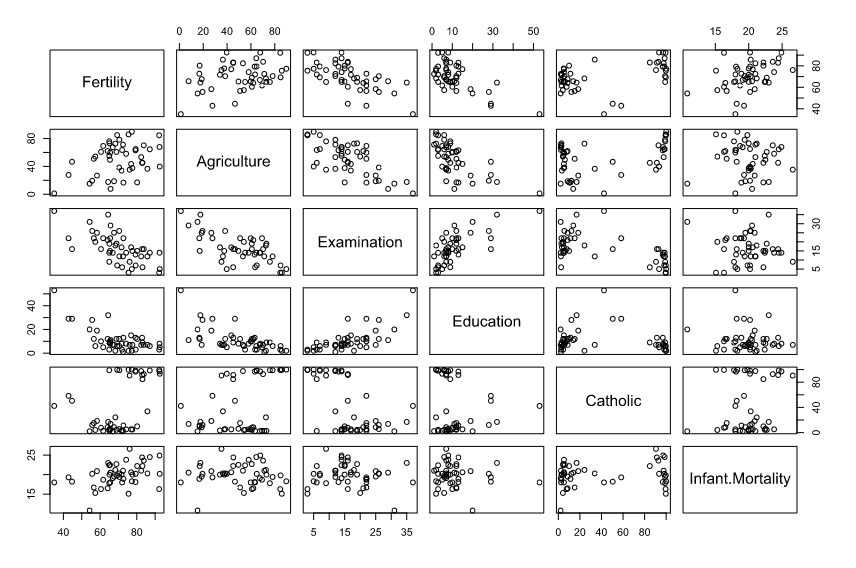
\includegraphics[width=0.8\linewidth]{Pairs}
\caption{Pairs Plot of Explanatory Variables}
\end{figure}


\noindent The Catholic variable is highly bimodal, with only a few points lying between the extremes of a majority Catholic or majority Protestant. Highly Catholic regions are typically less educated, score lower on the physical examinations, and are more agrarian. Given these extremes we decided to translate the Catholic variable into a categorical variable.\\

\noindent We note that Agriculture and Examination seem  slightly collinear. Similarly, we notice that Examination and Education exhibit the same behaviour. We will keep this is mind later once we begin reducing the number of variables in our model.

\section*{Fitting A Linear Model}

\noindent In order to determine possible data transformations, interactions, and variable selection, an initial linear fit of all explanatory variables is necessary. A multiple linear regression in RStudio yields the following output:

\begin{figure}[h!]
\centering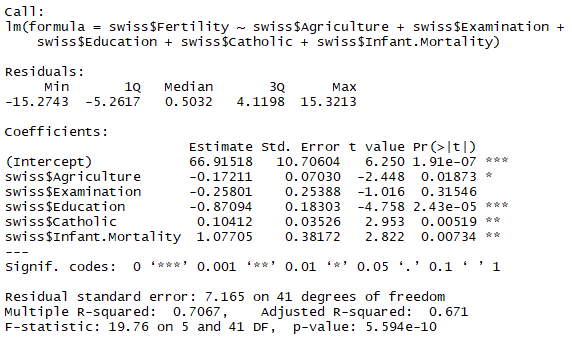
\includegraphics[width=0.7\linewidth]{SummaryBaseModel}
\caption{Summary Statistics for Base Model}
\end{figure}

\noindent We can see that Examination does not immediately seem statistically significant. This makes sense, as we previously noted that Examination and Agriculture seem slightly collinear. For this reason, we remove the Examination variable from our model and see the following results:

%Furthermore, one can notice that the relationship between Fertility and Examination in Figure 1 does not seem linear - it tends to behave similarly to an inverse function. For these reasons, a transformation of the Examination variable is considered: we attempt to fit another linear model with the new Examination variable \texttt{1/DenomExam}:

\begin{figure}[h!]
\centering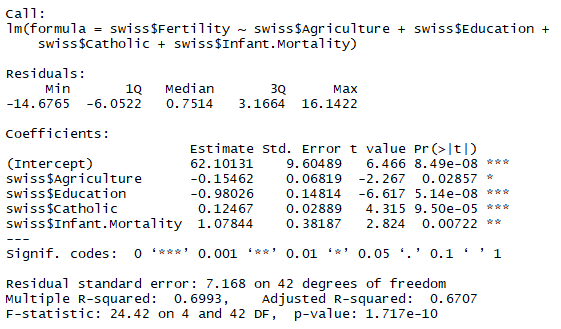
\includegraphics[width=0.7\linewidth]{SummaryStatsDenom}
\caption{Summary Statistics for Modified Base Model}
\end{figure}

\noindent In doing so, we ensure that all included parameters are statistically significant- that is, strengthening the global null hypothesis that all included parameters are non-zero. We do not, however, improve our adjusted R-squared value. Furthermore, removing the Agriculture variable does not marginally improve the fit of our model - our initial hypothesis that Agriculture and Examination are slightly collinear is either incorrect or relatively unimportant. Even though removing Agriculture improves the significance of all remaining parameters, Agriculture is itself significant enough to warrant inclusion. \\

\begin{figure}[h!]
\centering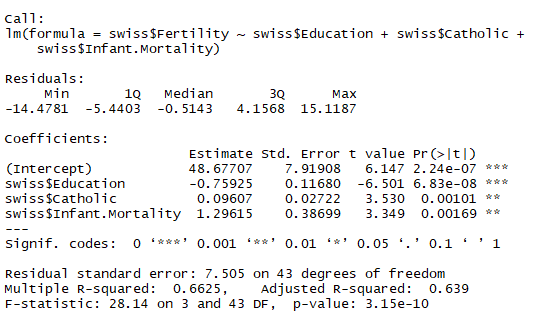
\includegraphics[width=0.7\linewidth]{SummaryStatsNoAgEx}
\caption{Summary Statistics for Modified Base Model, No Agriculture}
\end{figure}

\noindent Now that we have created an otherwise satisfactory model, we consider variable transformations. By plotting residual vs. fitted values for simple linear regression models of Fertility and Education, Agriculture, Catholic, and Infant.Mortality, respectively, we see the following results:

\begin{figure}[htp]
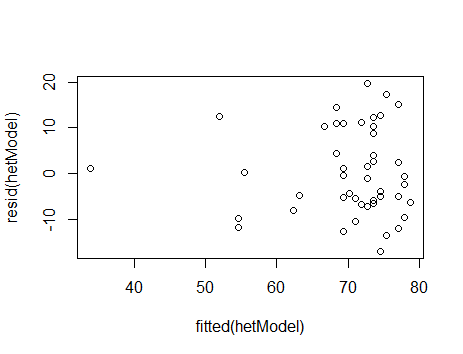
\includegraphics[width=.5\textwidth]{homoFertEdu}\hfill
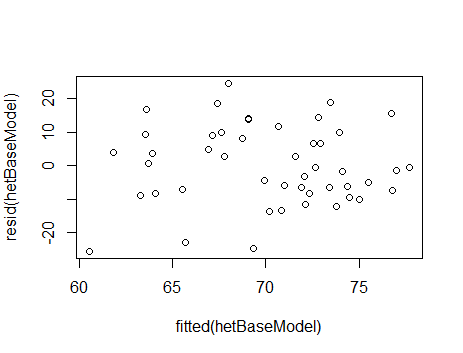
\includegraphics[width=.5\textwidth]{homoFertAg}
\caption{Checking Homoscedasticity - Education and Agriculture}
\end{figure}

\newpage

\begin{figure}[htp]
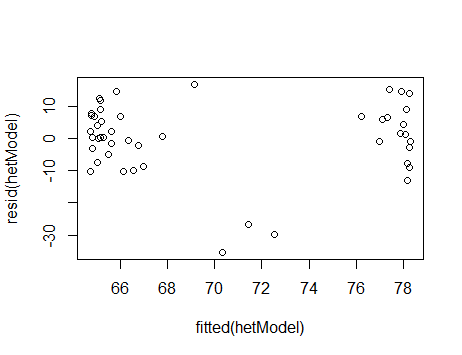
\includegraphics[width=.4\textwidth]{homoFertCath}\hfill
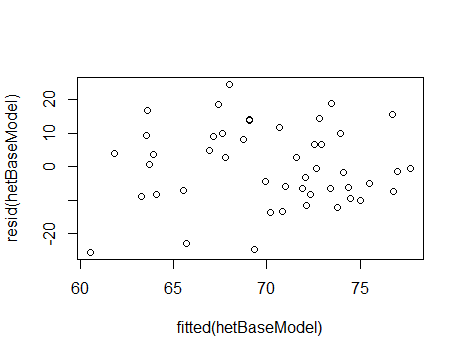
\includegraphics[width=.4\textwidth]{homoFertMort}
\caption{Checking Homoscedasticity - Catholic and Infant.Mortality}

\end{figure}

\noindent Notice that all of our data is relatively homoscedastic, with the relative exception of Education and Catholic: our Education variable has one outlier, but is otherwise fine; Catholic, on the other hand, demonstrates strong bimodal behaviour towards either strongly Catholic or Protestant regions. While homoscedasticity isn't necessarily violated here, it is worthwhile to see if creation of a categorical variable (either Catholic or not) could help the situation. We categorize each region as Catholic if 75 percent or more of its population are Catholic. Otherwise, the region is considered not largely Catholic. The point 75\% was chosen to caputre all of the extremely Catholic in one group and the remaining groups into another. This stratification yields the following results:

\begin{figure}[h!]
\centering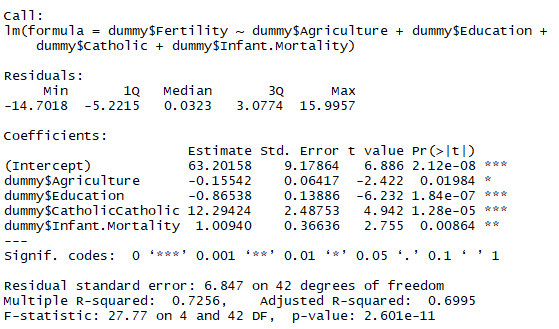
\includegraphics[width=0.7\linewidth]{SUmmaryStatsEndModel}
\caption{Summary Statistics for Modified Catholic Variable}
\end{figure}

\pagebreak

\section*{Leverage and Influence}

\noindent To determine if our model includes any high leverage points, we utilize RStudio's \verb|plot()| function to create a Residuals vs. Leverage plot, shown below. Since all points are within $\frac{1}{2}$ of Cook's distance, no points are influential in our model. Note however that two points have relatively high leverage compared to the rest of our data. Since both of these points agree on the fit of the model we can assume that they follow the same distribution of the rest of the data, so we can leave them in the model.

\begin{figure}[h!]
\centering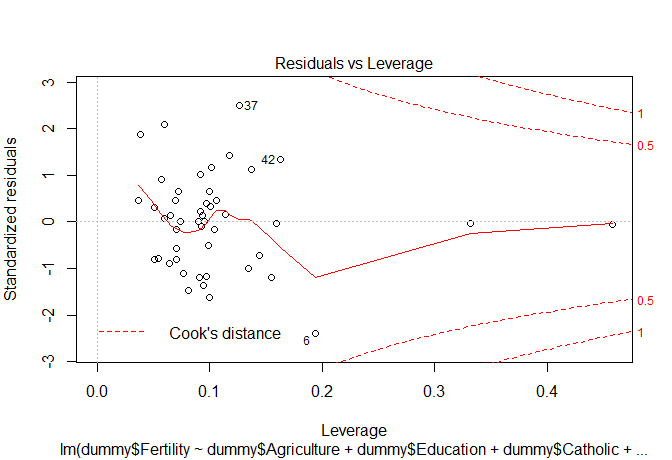
\includegraphics[width=0.7\linewidth]{Influentiality.PNG}
\caption{Influence of data points}
\end{figure}

\section*{Summary}
\noindent From our final model we can see that increase in agriculture corresponds to a small decrease in fertility. Education leads to a large decrease in fertility. In communities that we considered majority Catholic we saw a huge increase in fertility. Finally we see a increase in fertility with a near one-to-one scaling with infant mortality - clearly parents have a target number that they will reach, regardless of the failure rate. \\

\noindent Outside of the agriculture variable we see expected results. The agriculture variable was slightly collinear with examination. We believe that this discrepancy with our expectations comes from eligible males being drafted into the army given their high examination scores, leaving them unable to produce progeny during their prime years.\\
\newpage
\section*{Appendix of Code}

\noindent [1] Code for Base Model Creation
\begin{verbatim}
#generate linear model using all explanatory variables
baseModel = lm(swiss$Fertility ~ swiss$Agriculture + swiss$Examination 
    + swiss$Education + swiss$Catholic + swiss$Infant.Mortality)
summary(baseModel)
#create residual plots for Swiss Fertility and all variables in base model
hetBaseModel=lm(swiss$Fertility ~ swiss$Catholic)
\end{verbatim}

\noindent [2] Code for Reduced Model Creation
\begin{verbatim}
#generate linear model with reduced parameters
removedBaseModel = lm(swiss$Fertility ~ swiss$Education + swiss$Catholic 
    + swiss$Infant.Mortality)
summary(removedBaseModel)
\end{verbatim}

\noindent [3] Creation of Categorical Catholic Variable
\begin{verbatim}
#creates categorical catholic var
dummy = swiss
x = c()
for(i in 1:47) {
  if (dummy$Catholic[i] >= 75) {
    x[i] = "Catholic"
  }
  else {
    x[i] = "Average"
  }
}
dummy$Catholic = x
\end{verbatim}

\noindent [4] Generation of Final Model and Leverage Plot
\begin{verbatim}
#Code for End Model Generation
EndModel = lm(dummy$Fertility ~ dummy$Agriculture + dummy$Education 
    + dummy$Catholic + dummy$Infant.Mortality )
summary(EndModel)
#Decided this was the best music
hetEndModel=lm(dummy$Fertility ~ dummy$Catholic)
plot(fitted(hetEndModel),resid(hetEndModel))
plot(EndModel)
\end{verbatim}

\end{document}

%%
%% End of file `elsarticle-template-1-num.tex'.
